In this section we describe the experimental results we have obtained using Cerebro and the associated tools. We conduct
tests using five sample applications. 

\begin{description}
\item[StudentInfo] A JAXRS application for managing students of a class. Provides APIs for
adding/removing students, and listing the student information.
\item[ServerHealth] An application that monitors a given web URL for server uptime. Provides an
API for obtaining the uptime statistics computed by the application.
\item[SocialMapper] A simple social networking application. Provides APIs for adding users,
comments and other resources.
\item[StockTrader] A stock trading application. Provides APIs for adding users, registering
companies, buying and selling stocks among users.
\item[Rooms] A hotel booking application. Provides APIs for registering hotels and looking up
available rooms.
\end{description}

The above applications extensively use the datastore cloud SDK interface of Google App Engine. The Rooms application
additionally uses the memcache interface.

We instrument each of the five sample applications to measure the time taken by their web APIs to execute the
enclosed code. This is done by adding some extra Java code to each of the web APIs exposed by the sample applications.
We ensure that the instrumentation does not alter the original web API code in anyway (i.e. the original algorithms, control flow
and data flow are not impacted by the instrumentation). Then for each application we also
implement a mechanism to output the measured execution times, so an external client can query and collect the execution
times of the web APIs.

We carry out each of our tests in two separate environments -- Google App Engine public cloud, and
the AppScale private cloud. The AppScale private cloud used for testing was powered by four m3.2xlarge virtual machines 
running on a private Eucalyptus cluster.

In the first set of experiments, we benchmark each application for a period of 15 to 20 hours.
During this time we run an HTTP client on a separate machine that invokes the instrumented web APIs once every minute, 
and collects the server-side execution times (as measured by the instrumentation code).
At the same time, we also run Watchtower in the same target cloud environment as the sample application being tested to
benchmark the individual cloud SDK operations. Recall that our sample applications use datastore and memcache
cloud SDK interfaces. Hence
we configure Watchtower to periodically benchmark the cloud SDK operations related to these two interfaces. 
At the end of a benchmarking run, we have two sets of data at hand:

\begin{itemize}
\item Web API execution times collected by the benchmarking HTTP client
\item Cloud SDK benchmarking data gathered by Watchtower
\end{itemize}

We now run Cerebro to make predictions regarding the web API execution time using the cloud SDK benchmarking data
collected by Watchtower. We configure Cerebro to predict an upper bound for the 95th percentile of the web API
execution time, with an upper confidence of 0.01. Cerebro generates a sequence of execution time predictions -- one 
per minute. Then we compare these predictions against the actual web API execution times measured during the same
time period. More specifically, we approximately align the sequence of predictions with the time series of actual execution
time measurements, and check whether each prediction is equal to or higher than the corresponding measurement. We consider a 
sequence of 1000 consecutive predictions and 1000 consecutive API execution
time measurements, and compute the percentage of measurements that are less than or equal to the predicted values (a
metric that we sometimes refer to as \textit{percentage accuracy}).
 

\begin{figure}
\centering
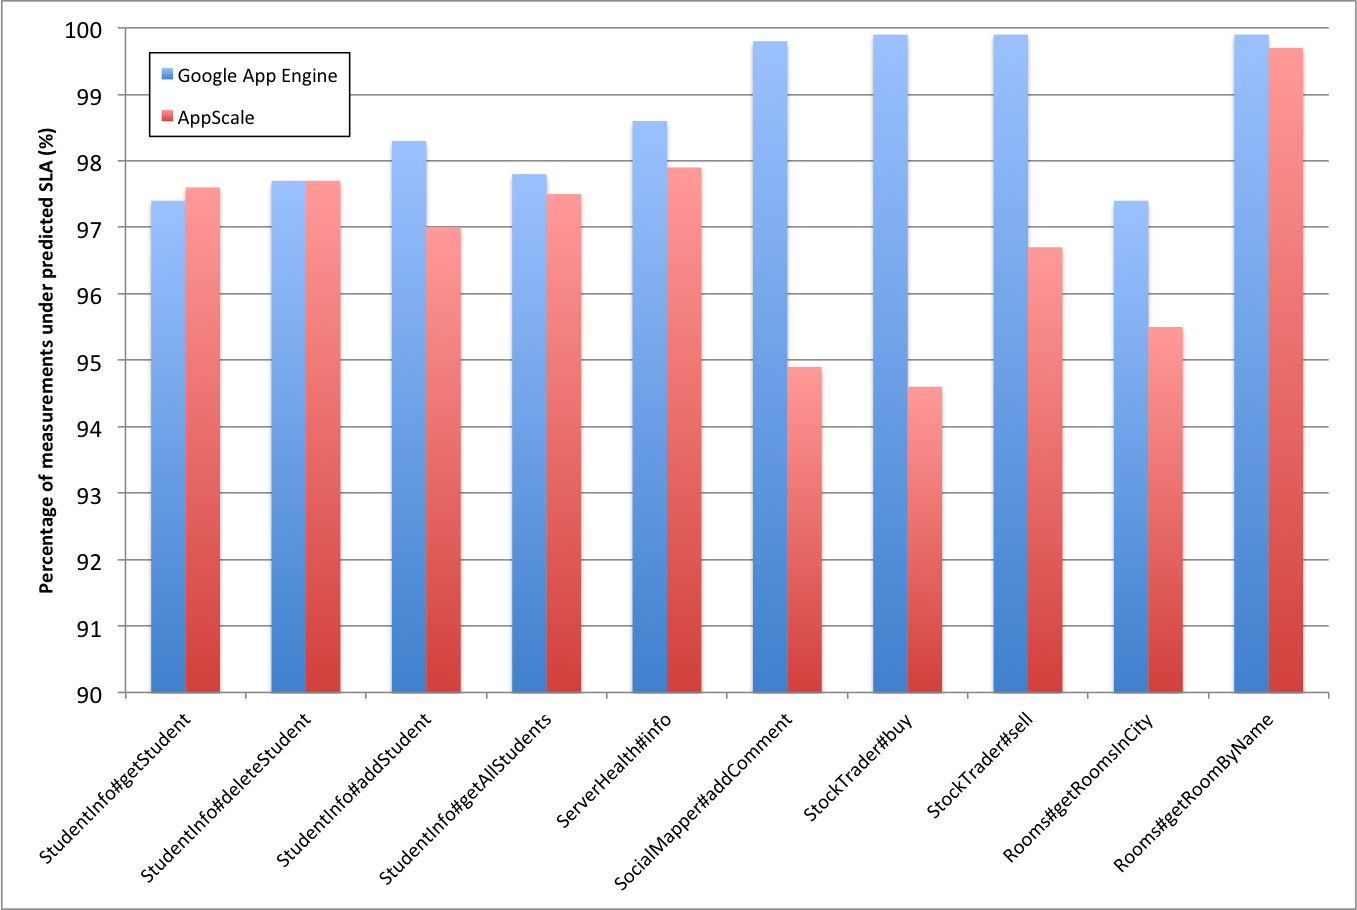
\includegraphics[scale=0.35]{accuracy_summary}
\caption{Percentage of measurements under predicted upper bound in Google App Engine and AppScale cloud platforms.}
\label{fig:accuracy_summary}
\end{figure}

Figure~\ref{fig:accuracy_summary} shows the final results of the above experiment.
Each of the columns in figure~\ref{fig:accuracy_summary} corresponds to a single web API operation in 
one of the sample applications. The columns are labeled in the form of \textit{ApplicationName\#OperationName} (a convention 
we will continue to use in the rest of the paper). To maintain clarity in the figures we do not 
illustrate the results for all web API operations in the sample applications. Instead we present the results for a selected set of 
web API operations covering all five sample applications. We note that other web API operations we tested also produce
very similar results.

Since we are using Cerebro to predict the 95th percentile of the API execution times, we expect approximately 95\% of the measured execution
times to be under the predicted upper bounds. According to figure~\ref{fig:accuracy_summary}, Cerebro achieves this goal for all
the cases considered in both Google App Engine and AppScale environments. The lowest percentage accuracy observed
in our tests is 94.6\% (in the case of StockTrader\#buy on AppScale), which is also very close to the target of 95\%. Such minor
lapses below 95\% are acceptable anyway, since we expect percentage accuracy value to be gently fluctuating around the
95\% mark over time (a phenomenon that will be illustrated in our later results). Overall, this experimental result shows us that
Cerebro produces highly accurate and reliable SLA predictions for a variety of applications running on two very
different cloud platforms.

The web API operations illustrated in figure~\ref{fig:accuracy_summary} cover a wide spectrum of scenarios that may be encountered
when statically analyzing web application code. StudentInfo\#getStudent and StudentInfo\#addStudent are by far the simplest
operations in the mix. They invoke a single cloud SDK operation each, and represent a simple datastore read scenario and a simple
datastore write scenario respectively. As per our survey on the cloud applications, these alone cover a significant portion of the 
web APIs developed for the Google App Engine and AppScale cloud platforms (1 path through the code, and 1 cloud SDK call). 
The StudentInfo\#deleteStudent operation makes two cloud SDK operations in sequence, whereas
StudentInfo\#getAllStudents performs a batch read from the datastore followed by a data dependent loop to iterate through the results.
In our experiment involving the StudentInfo\#getAllStudents operation, we had the datastore preloaded with 1000 student records, 
and Cerebro was configured to use a maximum entity count of 1000 when making predictions.

ServerHealth\#info invokes the same cloud SDK operation three times in sequence. Both StockTrader\#buy and StockTrader\#sell have
multiple paths through the code (due to branching), thus causing Cerebro to make multiple sequences of predictions -- one sequence
per path. The results shown in figure~\ref{fig:accuracy_summary} are for the longest paths which consist of seven cloud SDK invocations each. According to
our survey, 99.8\% of the execution paths found in Google App Engine applications have seven or less cloud SDK calls in them. Therefore we believe
that the web APIs in StockTrader application represent an important upper bound case. Rooms\#getRoomByName
invokes two different cloud SDK interfaces, namely datastore and memcache. Rooms\#getAllRooms is another operation that consists of
a batch read and a loop. In this case, we had the datastore preloaded with 10 entities, and Cerebro was configured to use a maximum entity
count of 10. It is indeed encouraging to see how Cerebro manages to produce highly accurate predictions for such a wide range 
of web API implementations and runtime scenarios on two cloud platforms.

\subsection{Tightness of Predictions}
In this section we discuss the tightness of the predictions generated by Cerebro. Tightness is a measure of how closely the predictions
reflect the actual response times of web APIs. This parameter is just as important as the percentage of measurements that fall under
the predicted SLA values (which 
was discussed in the previous section). Note that Cerebro can achieve a very high percentage accuracy level by simply generating a 
sequence of absurdly large predictions. But such results will obviously be of very little use to the cloud administrators and API
developers. For the predictions to be useful and even meaningful, they should be very close to the actual response times of the web APIs.

\begin{figure}
\centering
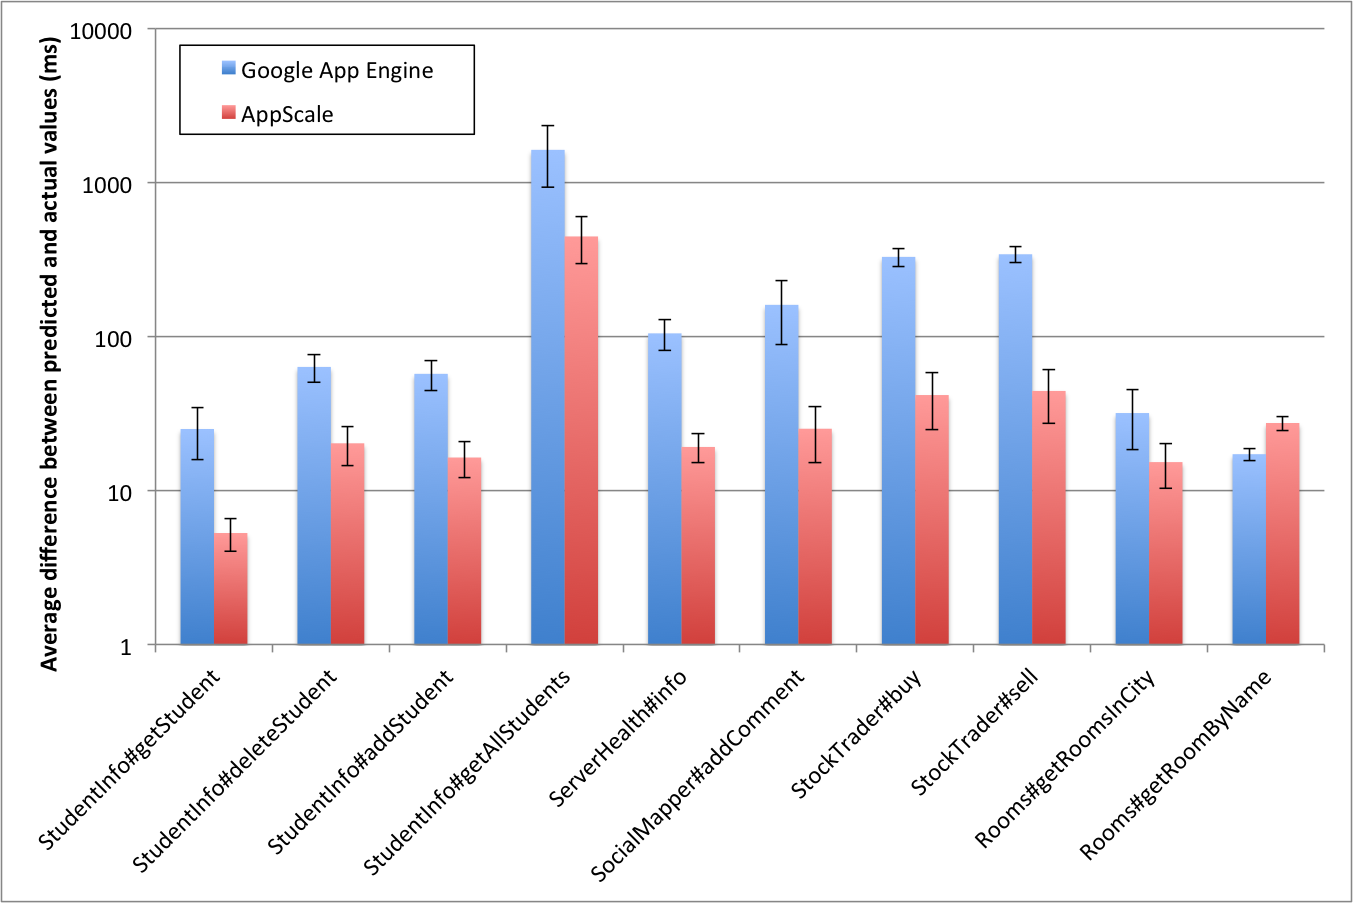
\includegraphics[scale=0.35]{diff_summary}
\caption{Average difference between predictions and actual response times in Google App Engine and AppScale. The y-axis is in log scale.}
\label{fig:diff_summary}
\end{figure}

Figure~\ref{fig:diff_summary} depicts the average difference between predicted response times and actual response times for
our sample web APIs when running in the Google App Engine and AppScale clouds. Note that the y-axis of the graph is
in log scale. These results were obtained considering a sequence of 1000 consecutive predictions (of 95th percentile) made by Cerebro. 
Within these prediction sequences only the cases 
where the predicted value was larger than the corresponding actual execution time was taken into account. Based on our previous results
regarding the percentage accuracy, we know that this case occurs approximately 95\% of the time.

According to figure~\ref{fig:diff_summary}, Cerebro generates fairly tight SLA predictions for most web API operations considered in the tests. In fact,
14 out of the 20 cases illustrated in the figure show average difference values less than 65ms. But for following scenarios Cerebro generated
predictions appear to be overly conservative:

\begin{itemize}
\item StudentInfo\#getAllStudents on both cloud platforms
\item ServerHealth\#info, SocialMapper\#addComment, StockTrader\#buy and StockTrader\#sell on Google App Engine
\end{itemize}

To understand why Cerebro generates conservative predictions for some operations we need to 
take a closer look at the performance characteristics of those operations. We take StudentInfo\#getAllStudents
operation on Google App Engine as a case study and analyze its execution time measurements in depth. 
Note that this is the case which exhibits the largest average difference between predicted and actual execution times.

\begin{figure}
\centering
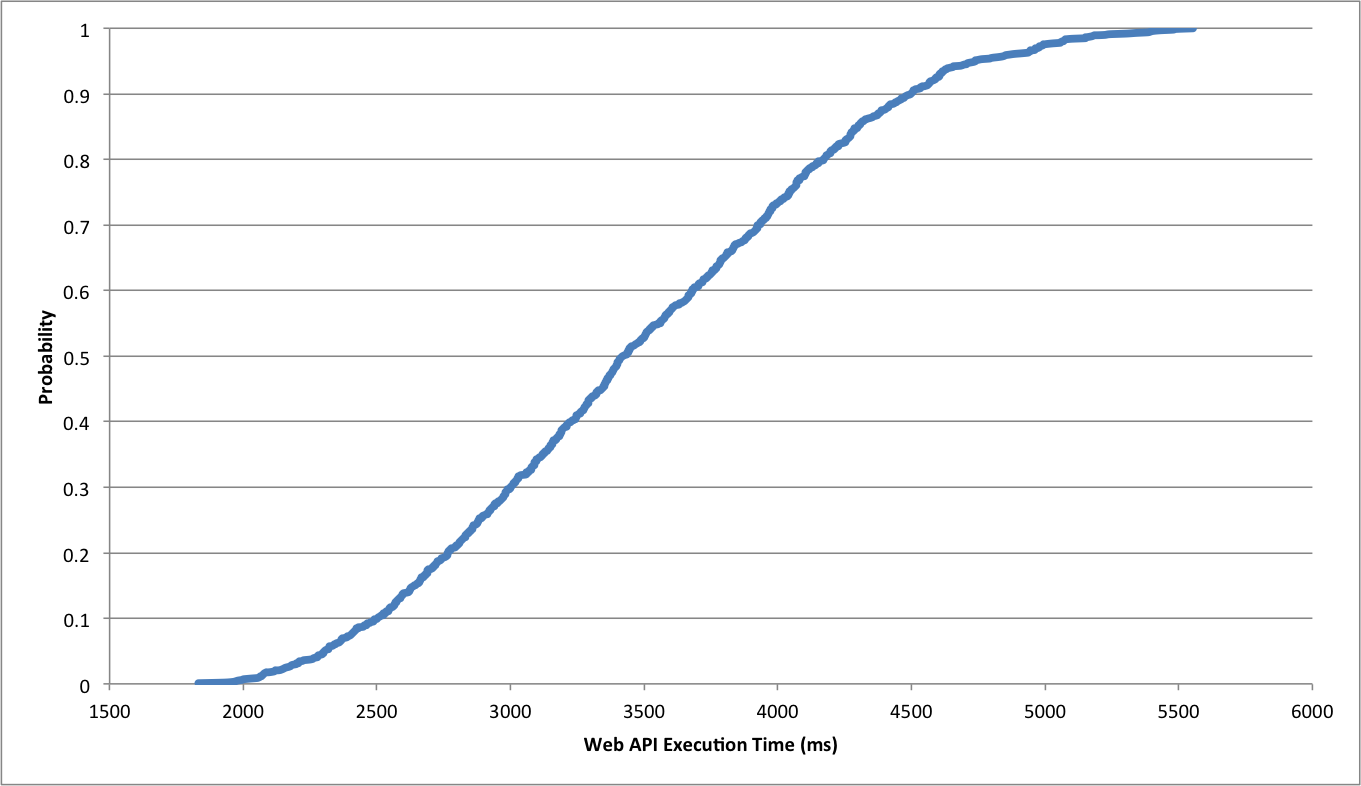
\includegraphics[scale=0.35]{get_all_students_cdf}
\caption{CDF of measured executions times of the StudentInfo\#getAllStudents operation on Google App Engine.}
\label{fig:get_all_students_cdf}
\end{figure}

Figure~\ref{fig:get_all_students_cdf} shows the CDF of measured execution times for the StudentInfo\#getAllStudents on Google
App Engine. This distribution was obtained by considering the benchmarking results gathered within a window of 1000 minutes. 
The mean and median of this distribution are 3431.79ms and 3383ms respectively. We make the following two observations from the
CDF:

\begin{itemize}
\item About 50\% of the values in the distribution are higher than the mean.
\item About 10\% of the values are higher than 4500ms; more than 1000ms higher than the mean.
\end{itemize}

These two facts indicate that the distribution of API execution times under consideration is significantly skewed away from its 
mean, and it is comprised of many high outliers (values that are significantly larger than the mean).
From this it becomes evident that StudentInfo\#getAllStudents operation records very high execution times frequently. 
In order to incorporate such high outliers, Cerebro must be conservative and predict large values for
the 95th percentile. This behavior is required to make sure that 95\% or more of the measurements fall under the
predicted values. However, as a consequence of this conservativeness the average distance between the measurements and 
the predictions is increased significantly. But all issues considered, the less tightness in the predictions made for StudentInfo\#getAllStudents
is not a limitation of Cerebro, but a feature necessary to guarantee the correctness of the results.

Our analyses with other operations for which
Cerebro generates conservative bounds have also shown similar results. That is, when the performance of the web API is highly variable and
when its execution time distribution contains
many high outliers, Cerebro produces predictions that are less tight. In other words, Cerebro trades off tightness of the predictions 
for their accuracy.

\begin{figure}
\centering
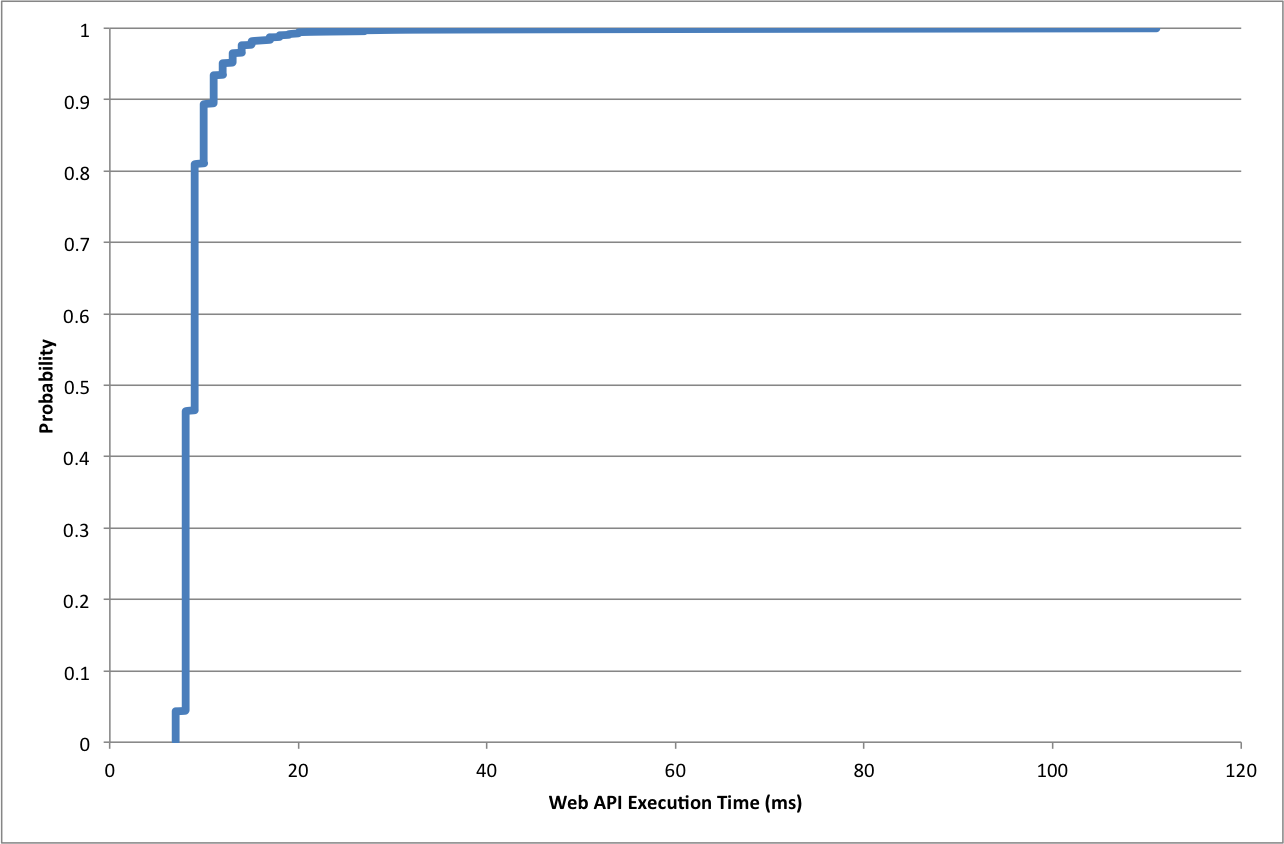
\includegraphics[scale=0.35]{get_student_cdf}
\caption{CDF of measured executions times of the StudentInfo\#getStudent operation on AppScale.}
\label{fig:get_student_cdf}
\end{figure}

To further reinforce this notion, we also take a close look at one of the web API operations that result in very tight predictions. 
Figure~\ref{fig:get_student_cdf} shows the CDF of the measured execution times for the StudentInfo\#getStudent operation on
AppScale cloud. Again we are considering a time frame of 1000 minutes when obtaining this graph.
This particular distribution has a mean of 9.19ms and a median of 9ms. Given that only 19\% of the values are larger than the mean, 
and only 2\% of the values are larger than 18ms (twice the mean), 
we see that this distribution is much more stable and have very few high outliers. This enables Cerebro to generate much
tighter predictions, without compromising the accuracy of the results. Based on these outcomes we can conclude that Cerebro produces
very tight upper bound predictions for web APIs whose performance is more stable over time. For APIs with highly variable performance
traits resulting in many high outliers, Cerebro generates more conservative and less tight predictions.

At this point it is worth reaffirming that Cerebro do not consider the actual execution time measurements of the web APIs when
making SLA predictions for them. It only has access to the cloud SDK benchmarking data gathered by Watchtower. We consider
Cerebro's ability to accurately determine the variability of a web API's performance by only looking at the cloud SDK
benchmarking data, to be one of its strengths.

Another interesting observation we can make regarding the tightness of the predictions made on our sample applications is that 
the predictions made in the AppScale cloud platform are significantly tighter than the ones made in the Google App Engine (figure~\ref{fig:diff_summary}). 
Five out of the six scenarios in which Cerebro has generated conservative predictions are from Google App Engine. Further
to that, for nine out of the ten operations tested, Cerebro has generated tighter predictions in the AppScale environment. This is 
because web API performance on AppScale is far more stable and predictable thus resulting in fewer high outliers in the corresponding
execution time distributions.

The reason why AppScale's performance is so stable over time is because it's a private cloud platform, deployed on a set of closely controlled 
and monitored cluster of VMs. We have total control
over how much resources are assigned to these VMs, and we ensure that they run in total isolation from the other processes running on the underlying hardware.
This is never the case when running our sample applications on Google App Engine, where we have no control over the underlying VMs, hardware and the
scheduling mechanism. Another related, but interesting outcome of these results is that large-scale public cloud platforms like Google App Engine, while
highly scalable, may not be able to support tight performance SLAs. Their performance is subject to high variations making it difficult to always support attractive
performance guarantees. Small private cloud platforms on the other hand can provide much better, consistent and stable performance guarantees, albeit their
poor scalability. From an organization's point of view this could be a strong motivator to adopt private cloud over public clouds.

\subsection{Accuracy Over Time and Convergence}
Earlier we looked at the percentage of measurements that are under predicted SLAs after a fixed amount of time has elapsed.
In those experiments we made predictions for a fixed-size time period (1000 minutes), 
and computed the percentage accuracy achieved by Cerebro at the end of the period.
In this section we are going to analyze the percentage accuracy of Cerebro as a running tabulation. That is, instead of just
computing the percentage accuracy at the end of 1000 minutes, we are going to compute it for each passing minute. This enables us to
understand how the percentage accuracy regarding a single web API operation changes over time, and the convergence
behavior of Cerebro.

\begin{figure}
\centering
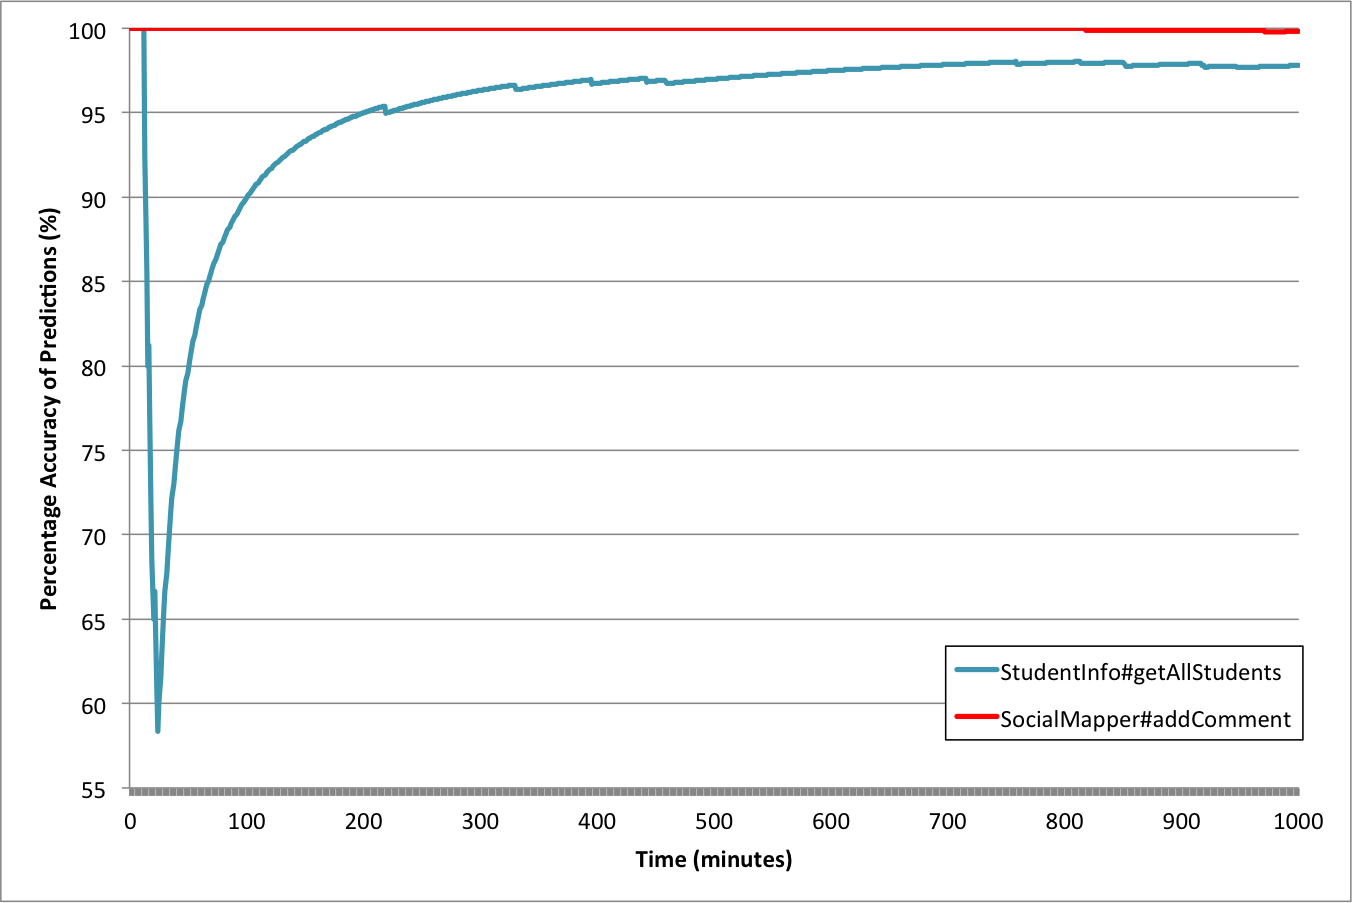
\includegraphics[scale=0.35]{gae_accuracy}
\caption{Percentage accuracy of predictions made on Google App Engine for a period of 1000 minutes.}
\label{fig:gae_accuracy}
\end{figure}

\begin{figure}
\centering
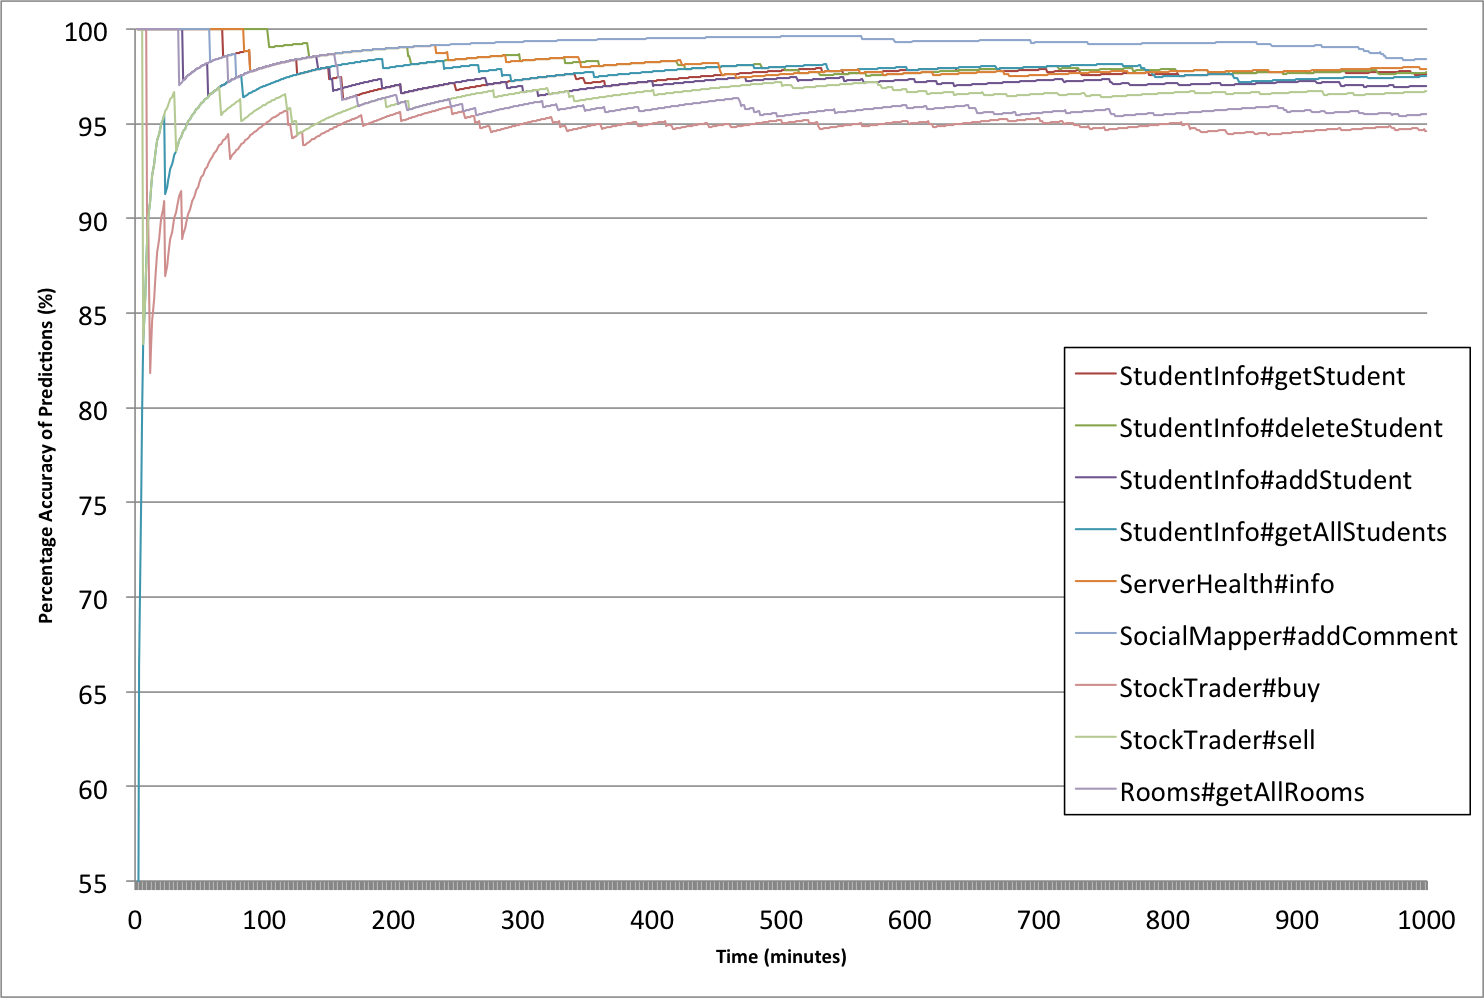
\includegraphics[scale=0.35]{as_accuracy}
\caption{Percentage accuracy of predictions made on AppScale for a period of 1000 minutes.}
\label{fig:as_accuracy}
\end{figure}

Figure~\ref{fig:gae_accuracy} shows the percentage accuracy of the Cerebro predictions made in the Google App Engine 
public cloud environment for a period of 1000 minutes. Each of the curves correspond to a single web API operation in one of the 
sample applications. 

As expected, the machine learning technique used by Cerebro takes some time to learn
from the time series data captured by Watchtower. This is when we see large fluctuations in the percentage accuracy. But
once Cerebro has converged it consistently produces highly accurate predictions regarding the 95th percentile of the web API
response time. In the worst case Cerebro takes up to 200 minutes to converge. This is the case with the
StudentInfo\#getAllStudents operation. After 275 minutes, we see highly accurate predictions being made on all web API
operations considered in the tests. After this point, we consistently see percentage accuracy values higher than 96\%. Note that
we had configured Cerebro to predict the 95th percentile of the web API executions time. Therefore as long as Cerebro produces
results with a percentage accuracy close to or higher than 95\%, we can consider the predictions to be correct and reliable.

Figure~\ref{fig:as_accuracy} shows the same results calculated by running Watchtower and the sample applications in the AppScale private cloud
environment. These results are very similar to the ones seen in Google App Engine, except for a somewhat faster convergence. In AppScale
we can see that Cerebro converges to the preferred percentage accuracy level in about 150 minutes.

An interesting observation we can make regarding the percentage accuracy over time is that it is never a constant function. 
Even after the percentage values have converged, they keep fluctuating 
around some median value. When the percentage accuracy starts to drop, Cerebro shifts the predictions up thereby increasing
the percentage accuracy. Similarly when the percentage accuracy increases, Cerebro shifts the predictions down. Due to this
continuous oscillation factor, we might encounter instantaneous percentage accuracy values that are slightly below 95\%. In fact this is exactly what is
happening with respect to the StockTrader\#buy operation in the AppScale environment. Its percentage accuracy converges to a median
value of 95\% and keeps oscillating around it. Therefore if we observe the instantaenous percentage accuracy of StockTrader\#buy at any given time, it
could be slightly above or below 95\%. But as long as this value does not diverge too far from 95\% mark, we can consider Cerebro predictions to
be accurate.

The key take away from the above results is that Cerebro needs to see cloud SDK benchmarking data for several hours (up to 200 minutes in case of 
Google App Engine), before it can start to produce stable and highly accurate SLA predictions. Therefore, it is a good idea to start Watchtower in the
target cloud platform early, and let it run for several hours before allowing API developers to deploy their web APIs on the cloud. Since the
required warm up period is in hours (as opposed to days or weeks), we believe this is a perfectly viable and reasonable solution to
ensure that any predictions made by Cerebro are up to the expected standards.

\subsection{Prediction Validity Period}
So far we have examined the accuracy, tightness and convergence behavior of the predictions produced by Cerebro. In this section we 
focus on the validity period of the Cerebro predictions.

Cloud platforms are highly dynamic environments. Some of the changes that may occur in such an environment are:
\begin{itemize}
\item addition or removal of hardware resources/VMs/containers,
\item software updates and upgrades, and
\item component failures.
\end{itemize}

When the platform is subject to such significant and frequent changes, any performance SLA predicted for a web API deployed on that
platform cannot hold correct forever. Given enough time, the APIs may start violating the predicted SLAs consistently. Therefore, for any
given SLA prediction we need to have an approximate idea of how long that prediction is going to be valid for. In others words, we need
to know how long it would take before a predicted SLA value cannot be considered correct. We refer to this time period as the validity
period of a prediction.

Ideally we want the validity period of a Cerebro prediction to be infinity. That is once an SLA prediction has been made for a web API it
should remain correct forever. If that was the case, the API performance would never degrade to a level where it
consistently exceeds the originally predicted execution time upper bound. But due to the dynamic nature of the cloud platforms such
behavior is highly unlikely. From a practical standpoint, we can expect the prediction validity period to be some finite duration. 

We believe
it is important that cloud administrators be informed about the validity period of predictions so that they can periodically reassess the web
API SLAs. For example they can run Cerebro periodically (before the prediction validity period expires) on the deployed web APIs to check
if the predicted execution times have degraded to such a level where they no longer meet the organizational standards for API
response times. If that is the case, the cloud administrators can take some remedial actions like committing more resources to the deployed APIs,
replicating them (horizontal scaling of the services), or notifying the respective API developers about the impending performance issues. However,
for this to be practical, the validity period of Cerebro predictions should at least be several hours. If the validity period is in the order of minutes,
a lot of computing time and manpower will be wasted recomputing Cerebro predictions and evaluating the results. Also, given that
modern cloud platforms are used to host thousands of web APIs, such aggressive recomputation of Cerebro predictions may not be scalable.

Before we can analyze the validity period of Cerebro predictions, we need to develop a precise model for detecting when a predicted SLA
has become invalid. Suppose at time $t$ Cerebro predicts value $Q$ as the $p$-th percentile of some API's execution time.
This means, if $Q$ is in fact a correct SLA prediction, the probability of API's execution time being less than or equal to $Q$ would be $0.01p$. 
Alternatively, the probability
of API's execution time being higher than $Q$, or the probability of API violating the predicted SLA is $(1-0.01p)$. By the same logic, 
the probability of API violating the predicted SLA $n$ times in a row is $(1-0.01p)^n$, if $Q$ is a valid prediction. 
Therefore, if we state that the 
predicted SLA is invalid, after observing $n$ consecutive violations, the probability of us being correct would be $1 - (1-0.01p)^n$. 
Notice that this value increases with $n$. 

This implies that we can use consecutive SLA violations by the API as an indicator of the SLA becoming
invalid. Larger the number of consecutive violations we observe, more confident we can be about categorizing the SLA as invalid. 
Hence for some $n$, if we observe
the $n$-th consecutive violation at time $t^\prime$, we can consider the duration $t^\prime - t$ as the validity period of the prediction made 
at time $t$. By the previous argument, the probability of this being an accurate approximation of validity period is $1 - (1-0.01p)^n$.

Lets consider a concrete example to further clarify this model. Assume that for some web API at time $t$ Cerebro produces value $Q$ as the 
prediction of the 95th percentile. Therefore after time $t$, the probability of the API violating this predicted SLA would be 0.05 (assuming $Q$ is
a correct SLA). The probability of the API
violating the SLA 3 times in a row is $0.05^3$ or 0.000125. At this point if we conclude that the predicted SLA is invalid, the probability of us
being correct is $(1 - 0.000125)$ or 0.999875. If we want to be even more confident about detecting SLA invalidations, we can look for even higher
number of consecutive SLA violations (i.e. higher $n$). This model enables cloud administrators to choose how certain they need to be about
considering a predicted SLA as invalid. Based on the value they choose for $n$ the validity period of the predictions can be determined
with a specific level of certainty.

To evaluate the validity period of Cerebro predictions, we benchmark some of our sample applications for a period of 5 to 6 days on both
Google App Engine and AppScale. We also run Watchtower on the same cloud platforms during this period. We run Cerebro using
the Watchtower data to make per-minute SLA predictions (95th percentile) for the entire duration of the tests. Then we choose a sequence of predictions
in 15 minute intervals. For each of the selected predictions we try to find the time until 3 consecutive violations by scanning ahead into the trace of
actual execution times gathered by directly benchmarking the web APIs. This provides us with a distribution of times to 3 consecutive SLA violations.
Interestingly, for some predictions we are not able to find to 3 consecutive violations in the traces of actual API execution times. We include
such cases in the distribution by right censoring. That is we consider the end of trace as the time to 3 consecutive violations for such cases.

\begin{figure}
\centering
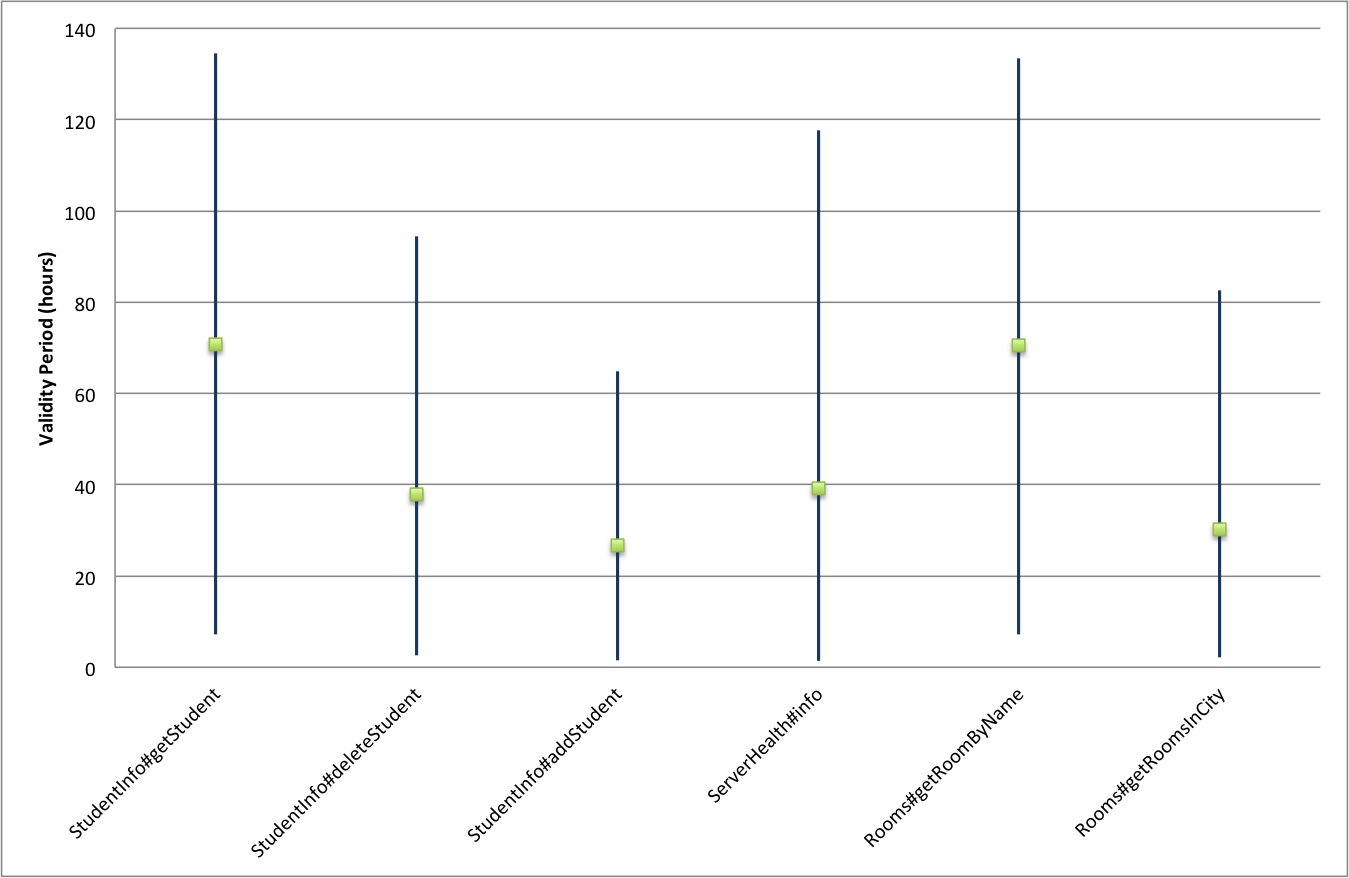
\includegraphics[scale=0.35]{gae_validity}
\caption{Prediction validity period distributions of different operations in Google App Engine. The vertical lines indicate the range between the 5th and 95th percentiles of the 
distributions. The green markers represent the means.}
\label{fig:gae_validity}
\end{figure}

\begin{figure}
\centering
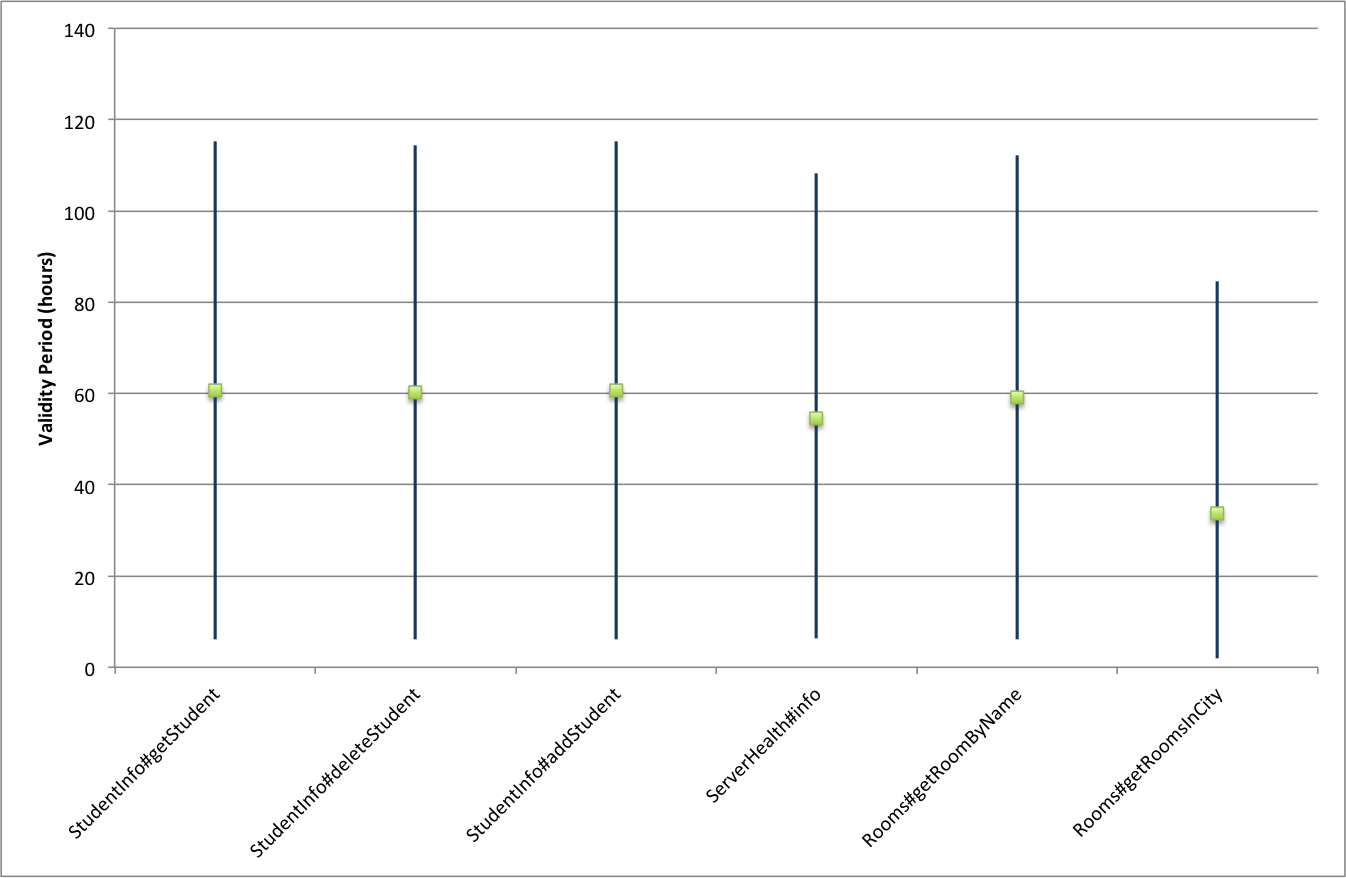
\includegraphics[scale=0.35]{as_validity}
\caption{Prediction validity period distributions of different operations in AppScale. The vertical lines indicate the range between the 5th and 95th percentiles of the 
distributions. The green markers represent the means.}
\label{fig:as_validity}
\end{figure}